\documentclass[letterpaper]{physor2024}

%%% Packages Required by Class (already included)
% fancyhdr
% lastpage
% titling
% titlesec
% ragged2e
% enumitem
% amsmath
% graphicx
% geometry
% newtxtext
% newtxmath
% hyperref
% cleveref
% caption
% authblk
% apptools
% appendix
% ifpdf
% epstopdf

%%% Some other useful packages
% \usepackage{tikz}
% \usepackage{color}
% \usepackage{subcaption}
% \usepackage{algcompatible}
% \usepackage{bm}
% \usepackage{array}

% GLOSSARIES
\usepackage[acronym,nomain,nonumberlist,nogroupskip,nopostdot]{glossaries} % for glossary of acronyms
\setacronymstyle{long-short}
\loadglsentries{glossary}
\makeglossaries
% \renewcommand*{\glstextformat}[1]{\textcolor{black}{#1}} % make glossary color black

% % This file contains custom commands that Lewis uses frequently in LaTeX documents

\usepackage{subcaption}
\usepackage{hyperref}
\hypersetup{colorlinks,allcolors=black}
% % for more https://tex.stackexchange.com/questions/88400/hyperref-changing-the-linkcolor-locally-in-the-toc

% custom equation commands
\newcommand{\QOR}{\qquad \text{OR} \qquad}
\newcommand{\QAND}{\qquad \text{AND} \qquad}
\newcommand{\QTHUS}{\qquad \text{THUS} \qquad}
\newcommand{\QWITH}{\qquad \text{WITH} \qquad}
\newcommand{\QFOR}{\qquad \text{FOR} \qquad}
\newcommand{\QSO}{\qquad \text{SO} \qquad}
\newcommand{\QWHERE}{\qquad \text{WHERE} \qquad}
\newcommand{\QWHEN}{\qquad \text{WHEN} \qquad}
\newcommand{\LINE}{\par\noindent\rule{\textwidth}{0.4pt}\par}
\newcommand{\toinf}{\rightarrow\infty}
\newcommand{\tozero}{\rightarrow0}
\newcommand{\qeq}{\overset{?}{=}}
\newcommand{\ceq}{\overset{\checkmark}{=}}
\newcommand{\Poi}{\text{Poisson}}
\newcommand{\keff}{$k_{e\!f\!f}$}
\newcommand{\kinf}{$k_{\!i\!n\!f}$}
\renewcommand{\epsilon}{\varepsilon} % squiggly epsilon

\def\brac#1{\{#1\}}
\def\Brac#1{\big\{#1\big\}}
\def\BRAC#1{\bigg\{#1\bigg\}}
\def\angbrac#1{\langle#1\rangle}
\def\Angbrac#1{\big\langle#1\big\rangle}
\def\ANGBRAC#1{\bigg\langle#1\bigg\rangle}
\usepackage{float}
\usepackage{multirow} % for special table
% % SI Units
\usepackage{siunitx}
\DeclareSIUnit\n{n}
\DeclareSIUnit\sp{sp}
% \title{OpenMC Depletion Analysis of a TRISO Fueled, Helium Cooled Microreactor}
\title{Exploring Effects of Homogenization on OpenMC Depletion Analysis of a TRISO Fueled, Helium Cooled Microreactor}

\addAuthor[ligross@wissc.edu]{Lewis I. Gross}{1}
\addAuthor{Benjamin Lindley}{1}
\addAuthor{Paul P.~H. Wilson}{1}

%%% Affiliations (from authblk)
%%% \addAffiliation{affiliationNumber}{Name of Institute, City, State/Country}
\addAffiliation{1}{University of Wisconsin - Madison, Madison, Wisconsin}

%%% Write text for abstract
%%% Most text modifying commands will work in abstract
\Abstract{OpenMC is a state-of-the art, open-source Monte Carlo transport code. This work uses OpenMC for depletion analysis of an infinite, unit cell model of the Virtual Test Bed gas-cooled microreactor. This microreactor is prismatic, TRISO-fueled, and helium gas cooled. Since the gas-cooled microreactor is intended for load-following, a depletion analysis was run at 100\%, 50\%, and 10\% of the rated power (225 kWt) for both explicitly represented TRISO and volume-homogenized fuel cases. \textbf{The time steps selected ensure the same total burnup at each step between power levels.} The system eigenvalue \kinf~was computed at each burnup step. The isotopics after one year of operation at steady-state were compared at each power for both homogenized and explicitly represented TRISO.}

%%% List up to 5 keywords separated by a comma
\keywords{OpenMC, TRISO, depletion, microreactor, gas-cooled}

%%% Provide a short title for the header on odd pages
\shortTitle{Depletion of a TRISO Fueled, Gas-Cooled Microreactor }

%%% Provide a short author listing for the header on even pages
\authorHead{Gross and Wilson}

%%% If LaTeX reports the line number of an error at \begin{document} it
%%%   is most likely due to an error in one of the commands above
\begin{document}

\section{INTRODUCTION}\label{sec:intro}
For advanced reactors, especially those early in the design stage, sufficient \gls{ms} are required to ensure the success of the design concept. Before any system can be built, modelers must prove systems perform safely. The \gls{vtb} \cite{vtb2023} is a repository of reactor models used for research and demonstration of current tools in the nuclear industry as a part of the \gls{neams} initiative. Various types of reactors are available on the \gls{vtb}. Microreactors are one viable class of next generation systems with ongoing modeling efforts using \gls{neams} tools \cite{Stauff-preliminary-applications-2021, Stauff-applications-2022}. One key advantage of microreactors is the ability to supply power to lower demand areas that may not be able to consume power on the order of a GW reactor or to areas needing temporary power, e.g.~natural disaster relief efforts. While microreactors can be diverse in fuel, coolant, and general design, there is interest in combining \gls{htgr} and microreactor technologies. \glspl{htgr} have the benefits of higher electricity conversion efficiency from higher temperature coolant plus the desirable melting properties of \gls{triso} fuel. Adding these benefits to a microreactor bring many attractive features together.

Previous work on the \gls{vtb} \gls{gcmr} includes analysis of the system for a two day load-following transient \cite{Abdelhameed-ANS-2022}. This work coupled Griffin, BISON, and SAM using the \gls{moose} framework. Griffin computed a solution to the neutron transport equation using a deterministic method, specifically the discrete ordinates and discontinuous finite element methods with the coarse mesh finite element method for acceleration. BISON is a fuel performance code that computed heat conduction in the solid parts of the system. SAM is a systems analysis code that computed heat transfer in the coolant channels.

Due to the smaller size of microreactors, it is conceivable to move the reactor at some point during operation, e.g. if the system was only needed temporarily or if power is needed elsewhere. In this case, for shielding and criticality safety reasons, the state of the core must be fully understood. If a system has been running on the order of months, the core composition has certainly changed since the initial loading due to the effects of depletion. Since Abdelhameed et al.~only modeled 48 hours, depletion was not considered. Any analysis occurring far enough into an operation cycle requires a burnup simulation to know the state of isotopics in the core, whether computing an accident source term or shielding requirements for transporting the reactor after a shutdown. A few depletion studies of other microreactor concepts exist, though this work adds the first depletion analysis to the \gls{vtb} \gls{gcmr}. A study of the gas-cooled, Japanese \gls{httr} computed criticality and burnup using various cross section representations with SCALE6 and MCNP5/X \cite{chiang-gcmr}. Another study looked at burnup for Westinghouse's eVinci \gls{hpmr}, finding that it could operate for at least 10 years without refueling, despite making more sense as a nuclear battery over a centralized power source \cite{Hernandez-hpmr}.

While previous work for the \gls{vtb} \gls{gcmr} used Griffin for neutron transport, this work chose OpenMC as an alternative to Griffin for a few reasons. First, OpenMC is an \gls{os} code. For this study, as well as others wishing to verify any OpenMC simulation, the code is freely available to use. As a Monte Carlo code, there are advantages over a deterministic code, like Griffin, for depletion analysis. The microscopic cross sections in continuous energy format are more accurate when modeling the resonance region, as opposed to representing them with multi-group cross sections. There's also no need to do smaller studies to compute fine or coarse-group cross sections to produce diffusion coefficients with transport corrections for leakage -- which is stronger in microreactors. OpenMC computes flux directly from continuous energy cross sections as an input to depletion.

The rest of this paper will be organized as follows. \cref{sec:depletion} will provide some background theory on depletion. \cref{sec:openmc_model}  will detail the \gls{vtb} \gls{gcmr} and its components, explaining the OpenMC model and the depletion schemes. \cref{sec:results} will present results for the system. \cref{sec:conclusions} will interpret those results and discuss the plans forward for more \gls{ms}.

\section{DEPLETION THEORY}\label{sec:depletion}
Once any reactor starts running, the composition of isotopes will change over time. Nuclides exposed to neutron flux will transmute into radioisotopes that have various modes of decay, creating new isotopes that did not exist at the start of operation, as well as decaying into other isotopes already in the system. The rate at which isotopes transmute and decay into each other depends on the transport solution via the reaction rates, which depend directly on the neutron flux. This relationship causes the coupling between transport and depletion to behave non-linearly \cite{romano-depletion-2021}.

Certain isotopes have more influence on the system than others. For example, Xenon-135 has an extremely high neutron absorption cross section. It is so high that its negative reactivity insertion influences the positioning of the control elements. Xenon-135 is particularly important in load-following contexts, in which the power changes once or twice per day, as it's concentration increases when power decreases, and it is burned off when power increases again. This matters more in load-following contexts because the Xenon-135 half-life is on the order of 9 hours \cite{d-and-h}. For context, the load following schedule in Abdelhameed et al. has high power for 12 hours, lower power for 7 hours, and 2.5 hour ramps between, inspired from the NEA OECD report on load-following \cite{Abdelhameed-ANS-2022,nea-oecd-LF}.

To model burnup, transmutation and decay cross sections of the isotopes are combined with the computed flux to determine production and destruction rates for each isotope. These formulate a system of differential equations for the nuclide densities. For isotope $i$ with number density $N_{i}(t)$, the Bateman or burnup equations describe the time dependent isotopic composition, given by

\begin{multline} \label{eq:batemen}
    \frac{dN_{i}}{dt} =
    \sum_{j} \bigg[f_{j\rightarrow{i}}\int_{0}^{\infty} \sigma_{j}(E,t)\phi(E,t)dE + \lambda_{j\rightarrow{i}}\bigg]N_{j}(t) \\
    -\bigg[\int_{0}^{\infty} \sigma_{i}(E,t)\phi(E,t)dE
    +\sum_{j}\lambda_{i\rightarrow{j}}\bigg] N_{i}(t),
\end{multline}

\noindent where $\sigma_{j}(E)$ is the transmutation cross section of isotope $j$ at energy $E$, $f_{j\rightarrow{i}}$ is the fraction of transmutation reactions for nuclide $j$ that produce nuclide $i$, and $\lambda_{j\rightarrow{i}}$ are the decay constants for decay modes in nuclide $j$ that produce nuclide $i$. The system of equations for isotopes $i\in[1,n]$ can be expressed in matrix notation using the nuclide vector $\mathbf{n}\in\mathbb{R}^{n}$
\begin{equation} \label{eq:burnup matrix odes}
    \frac{d\textbf{n}}{dt} =
    \textbf{A}(\textbf{n},t) \textbf{n}
    \QWITH
    \textbf{n}(0) = \textbf{n}_{0},
\end{equation}

\noindent where $\textbf{A}\in\mathbb{R}^{n\times n}$ is the burnup matrix. Since the transport equation depends on number density and $\textbf{A}$ depends on the solution to the transport equation, $\textbf{A}$ then also depends on number density. Because ``the timescale over which material compositions change is sufficiently long ... the transport equation can be solved as a steady-state equation" \cite{romano-depletion-2021}. Taking the burnup equations as quasi steady-state allows the earlier non-separable equation to be solved via separation solution
\begin{equation} \label{eq:separable burnup matrix odes}
    \frac{d\textbf{n}}{dt} =
    \textbf{A}(\textbf{n}) \textbf{n}
    \QWITH
    \textbf{n}(0) = \textbf{n}_{0},
\end{equation}

\noindent The solution to which is
\begin{equation} \label{eq:separation solution}
     \textbf{n}(t) = \exp(\textbf{A}t) \textbf{n}_{0}
\end{equation}

\noindent Solving \cref{eq:separable burnup matrix odes} and \cref{eq:separation solution} involves two separate components \cite{romano-depletion-2021}:
\begin{enumerate}
    \item Using a numerical method to integrate the matrix $\textbf{A}$ in \cref{eq:separable burnup matrix odes} forward in time. This usually involves taking one or more matrix exponential.
    \item Evaluating the matrix exponential $\exp(\textbf{A}t)$ or the action of the matrix exponential on a vector of nuclide concentrations.
\end{enumerate}

There are various methods for time integration. Predictor-Corrector methods are commonly used for time integration in burnup contexts. In this study, the second order \gls{cecm} is chosen, which is implemented by OpenMC and based on work comparing various integration schemes for depletion \cite{isotalo_comparison_2015}. Since the method is second order, it requires two transport solves per depletion time step: one for the prediction and one for the correction. Using appropriate time steps for the quasi static assumption of burnup is also important. Namely, using smaller time steps when nuclide concentrations are expected to be changing more rapidly and smaller time steps when nuclide concentrations are expected to be changing more slowly.

\section{OPENMC MODEL}\label{sec:openmc_model}
This section will describe the \gls{gcmr} system and the corresponding OpenMC model. There are two parts to the model. The first assembles the geometry and material definitions. The second takes this model as input and defines a depletion simulation, facilitating the alternating transport, depletion, and nuclide updates.

\subsection{System Description}\label{sec:system}
 \cref{fig:vtb_gcmr} shows a diagram of the \gls{gcmr}. The overall structural material of the unit cell is graphite, with cylindrical compacts arranged in a hexagonal lattice. The lattice's pitch is $2.00$ cm with the following compacts and their radii: burnable poison ($r=0.25$ cm), moderator ($r=0.95$ cm), coolant ($r=0.6$ cm), fuel ($r=0.9$ cm), and a central control rod ($r=0.99$ cm). The fuel kernel uses a U235 enrichment of 19.95\% inside the center of the \gls{triso} particles. The \gls{triso} has a $40\%$ packing fraction. The moderator uses YH$_{2}$ encased in a FeCrAl envelope ($0.05$ cm thick). The poison compacts contain B$_{4}$C burnable absorber spheres, which have a $25\%$ packing fraction. The coolant uses helium and the control rod chamber has a B$_{4}$C rod. Helium fills the space when the control rod is not fully injected; this helium is not circulating like the coolant. There is a top and bottom reflector made of BeO. Since the goal of this simulation is to determine excess reactivity in the system, the control rod is not inserted into the active core region, resting in the central compact of the upper reflector region \cite{Abdelhameed-ANS-2022}.
\begin{figure}[h!]
    \centering
    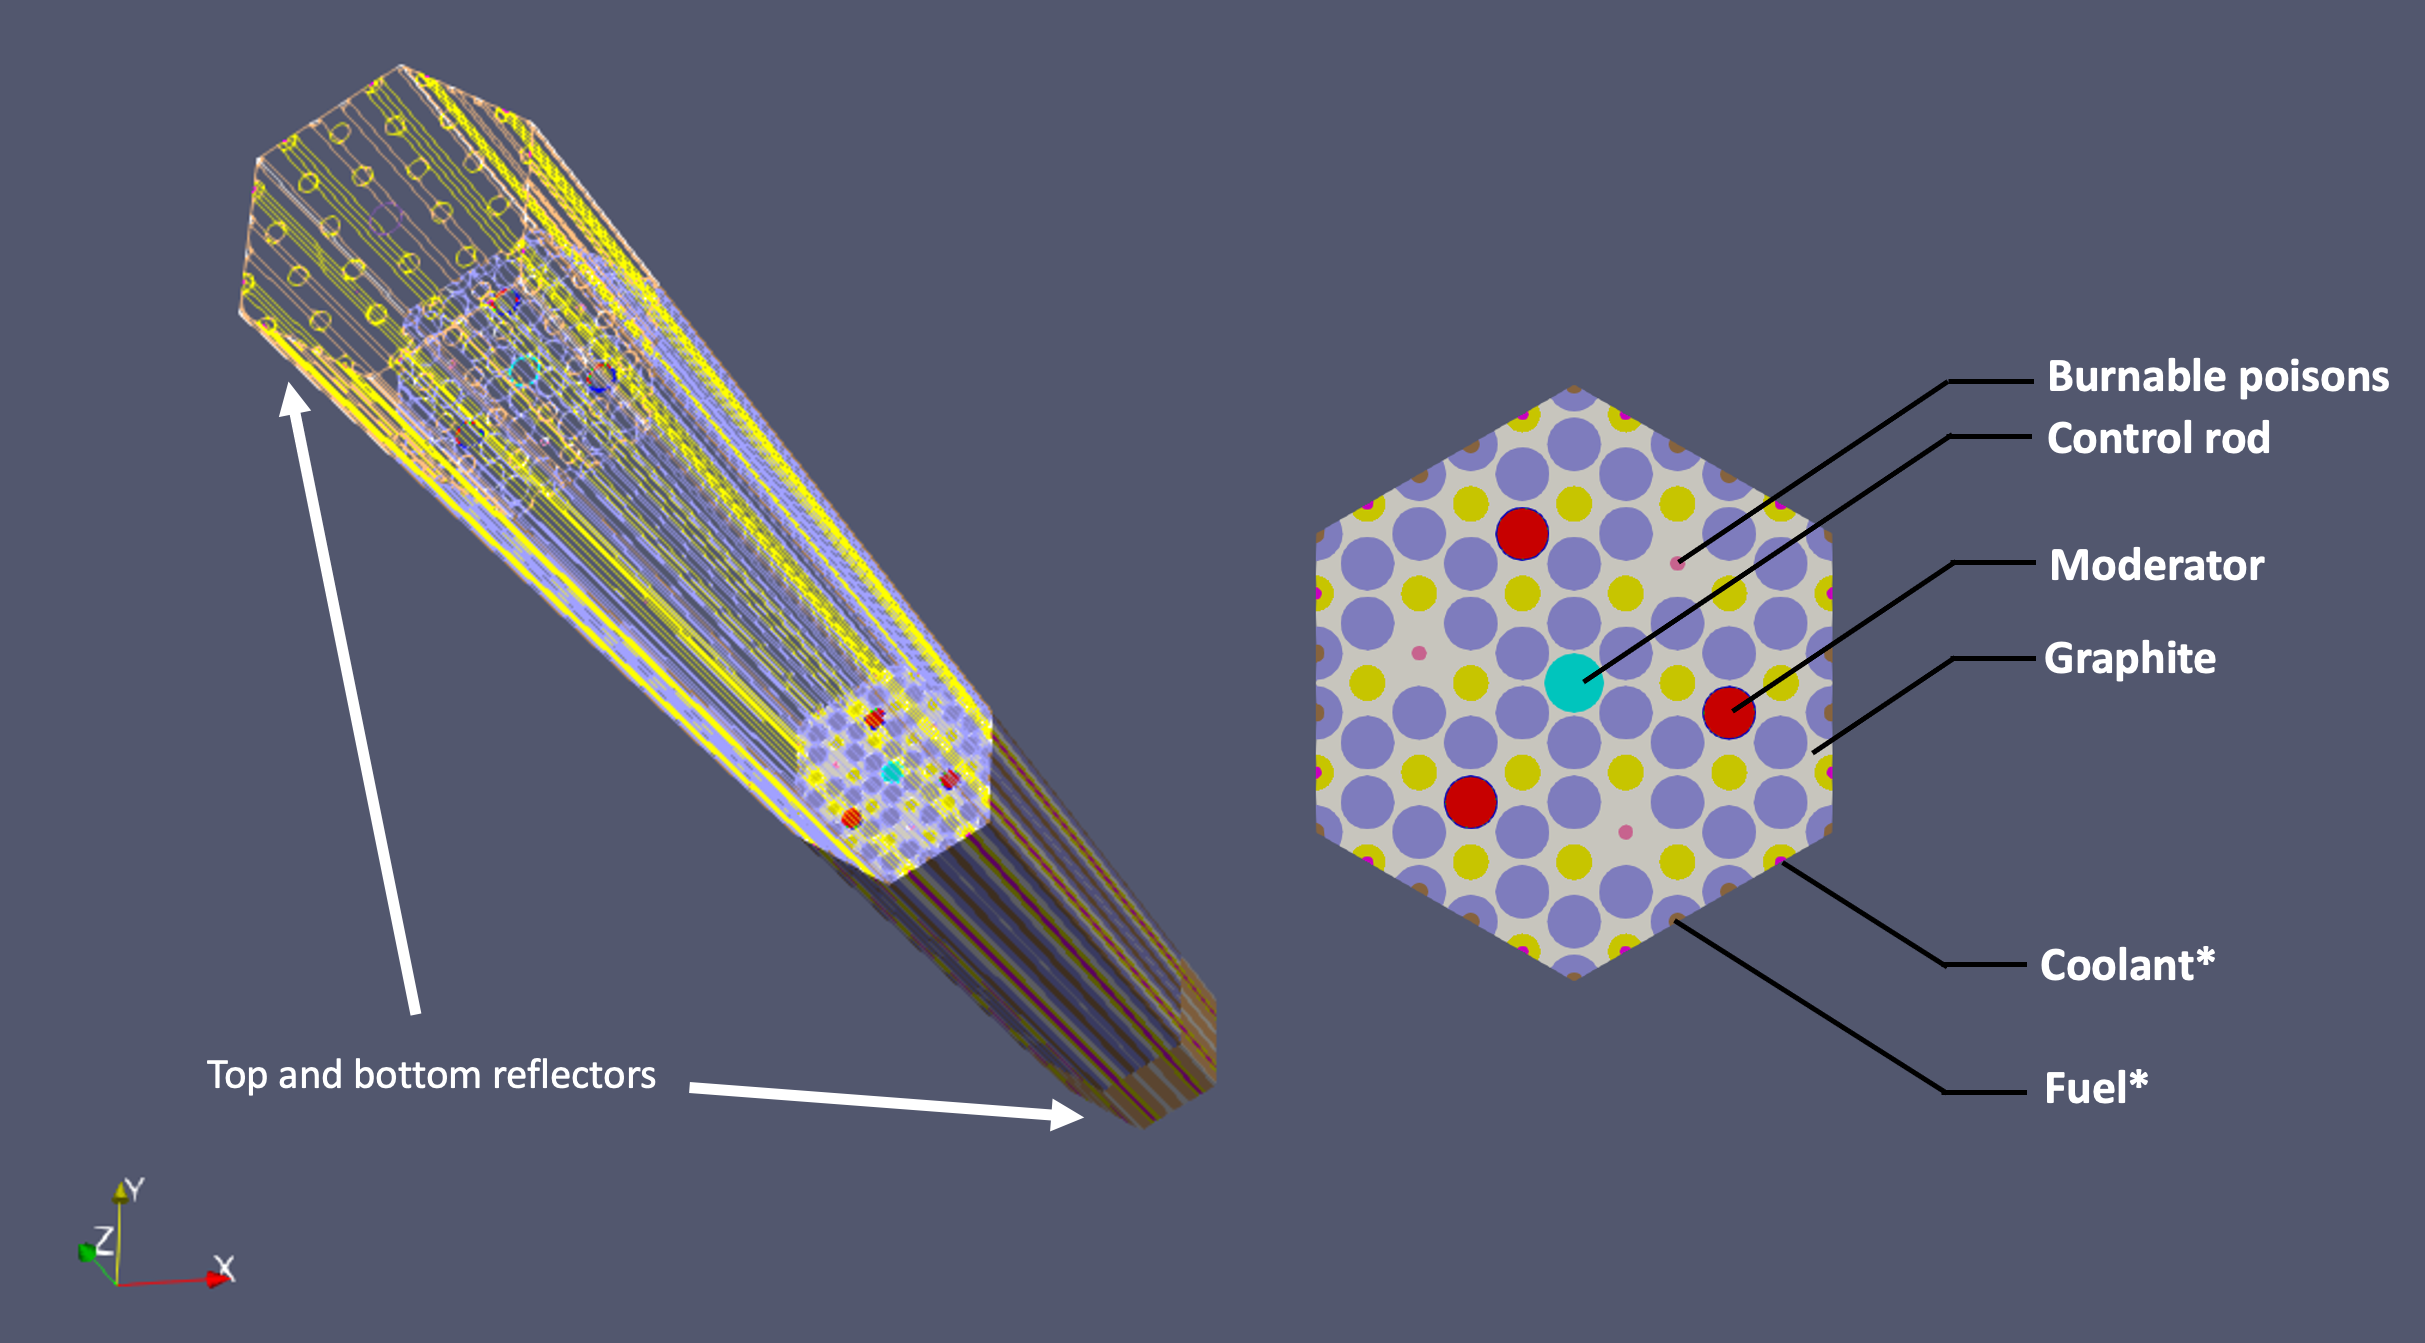
\includegraphics[width=0.9\linewidth]{figures/vtb_gcmr_diagram.jpg}
    \caption{An image of the \gls{vtb} \gls{gcmr} along with a cross section of the fuel containing section of the system.}
    \label{fig:vtb_gcmr}
\end{figure}

\subsection{Model Definition}\label{sec:model_def}
The system is divided into axial layers to compute spatial variation in flux. Since flux is a key input in to depletion, this allows depletion to also take advantage of the axial discretization and deplete at different rates accordingly. The axial division matched exactly the choice of \cite{Abdelhameed-ANS-2022}, which includes two regions per reflector and 16 regions in the active fuel region. The heights of each region are 20 cm for each reflector and 160 cm for the fuel, which corresponds to each axial layer modeling 10 cm of the reactor. \cref{fig:core_slice_sbs} shows a radial slice of the fuel portion of the reactor. \cref{fig:reflectors} shows a radial slice of each reflector region.

\begin{figure}[h!]
    \centering
    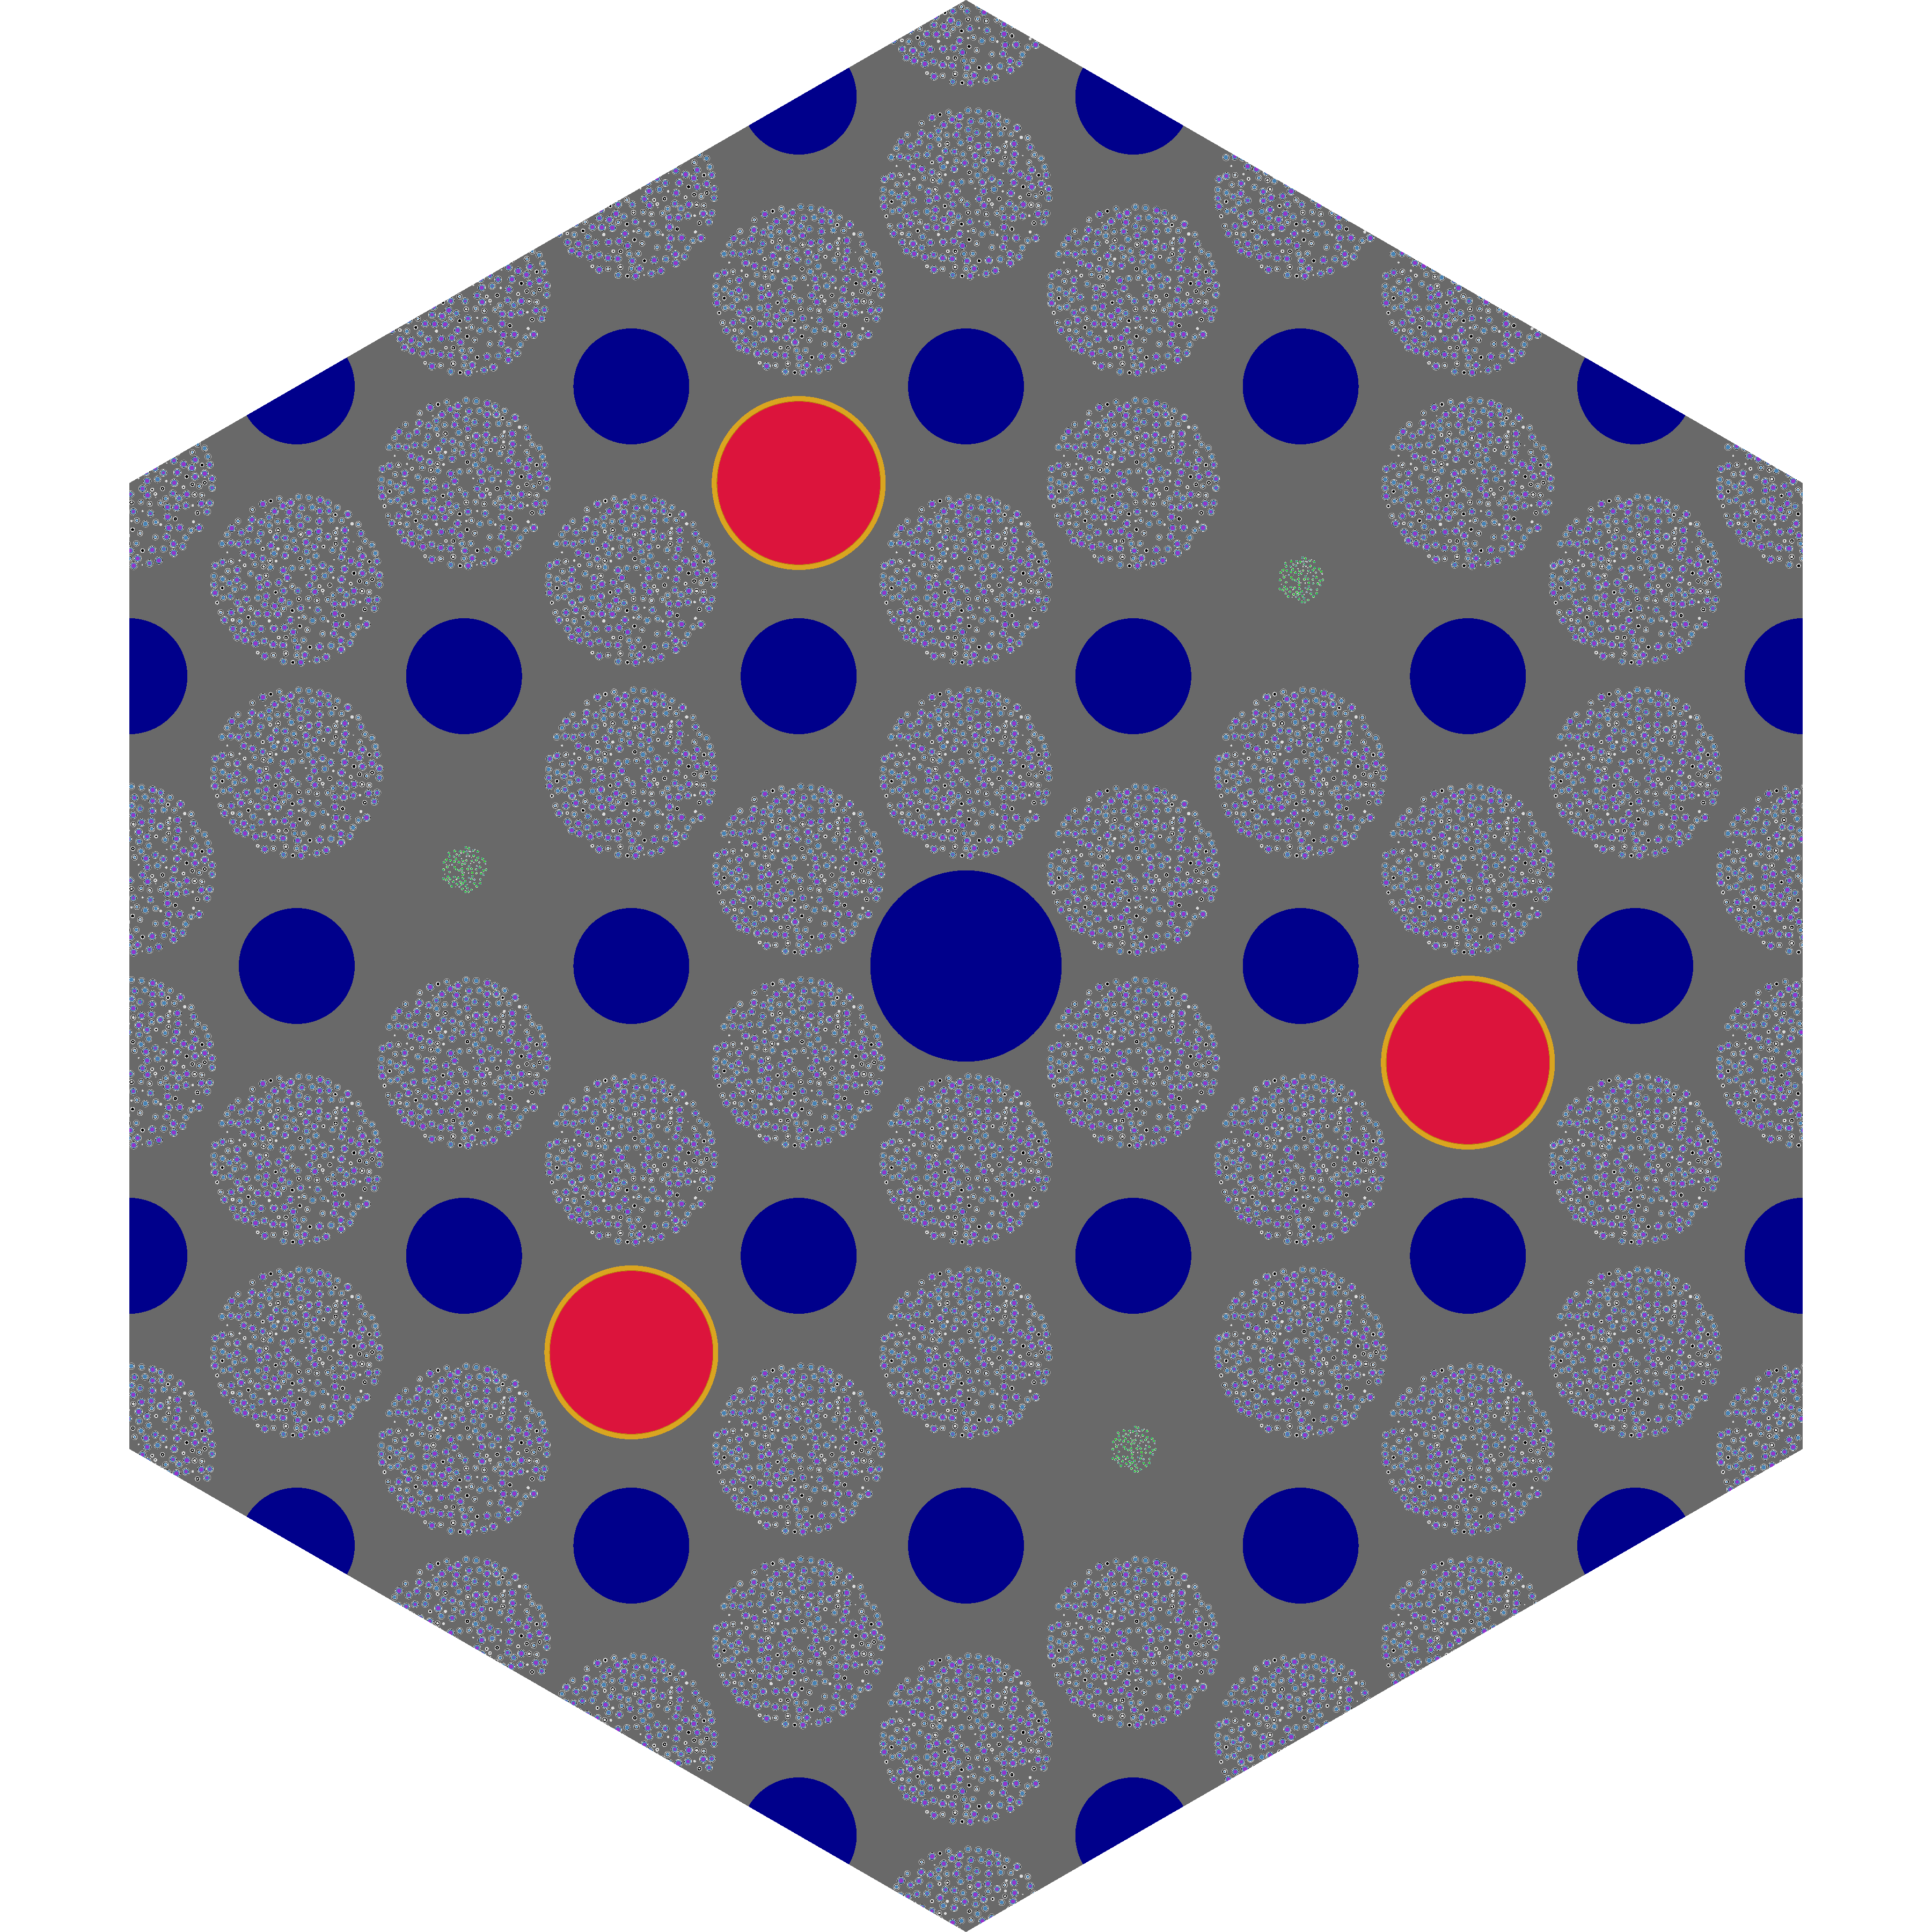
\includegraphics[width=0.525\linewidth]{figures/active_height.png}
    \label{fig:active_slice}
    \caption{A radial slice of the active region. Gray corresponds to graphite in the matrix or pyrolitic carbon, dark blue corresponds to helium coolant, red corresponds to YH$_{2}$ moderator, gold corresponds to FeCrAl, green corresponds to the B$_{4}$C poison particles (packed at 25 percent in graphite), and purple corresponds to the fuel kernel in the \gls{triso} particles (packed at 40 percent in graphite).}
    \label{fig:core_slice_sbs}
\end{figure}
\begin{figure}[h!]
    \centering
    \begin{subfigure}{0.49\linewidth}
        \centering
        
\includegraphics[width=0.825\linewidth]{figures/lower_reflector.png}
        \caption{A slice of the lower reflector, colored by material.}
        \label{fig:lower_reflector_slice}
    \end{subfigure}
    \begin{subfigure}{0.49\linewidth}
        \centering
        
\includegraphics[width=0.825\linewidth]{figures/upper_reflector.png}
        \caption{A slice of the upper reflector, colored by material.}
        \label{fig:upper_reflector_slice}
    \end{subfigure}
    \par\medskip
    \caption{A radial slice of the lower reflector (left) and the upper reflector (right). The difference between the upper and lower reflectors is that the upper reflector has an extra compact for the B$_{4}$C control rod. Dark blue corresponds to helium coolant
    and light blue corresponds to BeO, while the B$_{4}$C control rod is shown in green.}
    \label{fig:reflectors}
\end{figure}

\subsection{Depletion Simulation Definition}\label{sec:depl_sim}
With complete geometry and material definitions, the depletion simulation defines power history, time steps, and an integration scheme. OpenMC then alternates between transport and Batemen equation solves. The cross sections used for transport are continuous energy from ENDF-B-VII.1. The chain file, an XML file used for depletion in OpenMC, contains transmutation and decay data to compute the burnup matrix and each depletion time step. The chain file selected for this simulation is based on the \gls{casl} project. While the chain originates from a \gls{lwr} system, the similarity of the neutron spectrum, i.e. both thermal, makes this chain file a good choice, since $\phi(E)$ is one of the inputs when computing the burnup matrix. The \gls{casl} chain can be found on OpenMC's website, specifically the portion that provides data for users to download.

In this work, the system is held at constant power for each case. This has some implications for the time stepping scheme chosen. To correctly account for the rapid build up of strong neutron absorbers, a few short initial time steps are included to increase those nuclides' accuracy. The time steps can be lengthened after this initial transient behavior, after allowing these important isotopes to reach a steady-state. The time steps for the full power case, in days, were as follows: three one-day time steps, three five-day time steps, and 23 fifteen-day time steps.

\section{RESULTS}\label{sec:results}
There are a few metrics to compare between the different powers and TRISO representations. First, comparing the eigenvalue as a function of burnup gives a way to comapre the effect of homogenization.  \cref{fig:kinfvsburnup} shows results for the full power case of \kinf versus burnup for the time steps mentioned above. The full paper will show comparison for each lower power case as well.

\begin{figure}[!h]
    \centering
    \begin{subfigure}{0.49\linewidth}
        \centering
        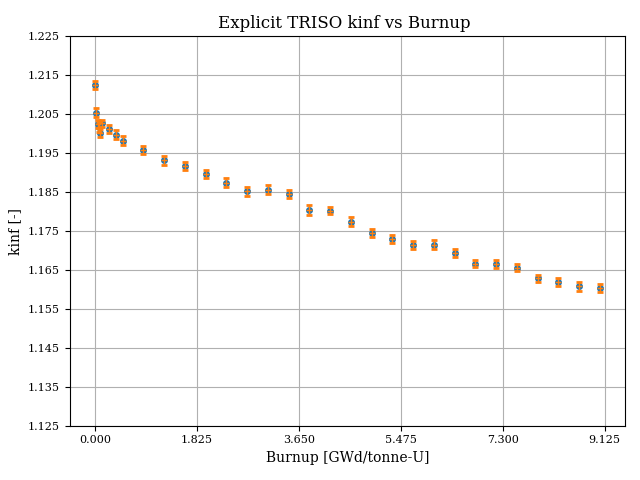
\includegraphics[width=\linewidth]{figures/explicit_kinf_vs_burnup.png}
        \caption{Explicit}
        \label{fig:explicit}
    \end{subfigure}
    \begin{subfigure}{0.49\linewidth}
        \centering
        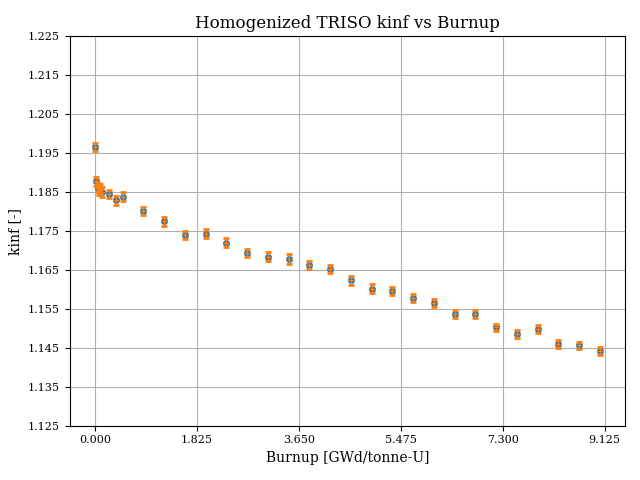
\includegraphics[width=\linewidth]{figures/homogenized_kinf_vs_burnup.png}
        \caption{Homogenized}
        \label{fig:explicit}
    \end{subfigure}
    \caption{Pictured above is results for \kinf versus burnup, both for the explicit \gls{triso} representation and homogenized fuel cases.}
    \label{fig:kinfvsburnup}
\end{figure}

The above results are in line with previous work measuring the effects of \gls{triso} homogenization. The explicit case has a noticeably higher eigenvalue. The eigenvalue increases for the \gls{triso} case due to the difference between neutrons interactions with the fuel. When the \gls{triso} is explicitly represented, neutrons slow down significantly more before hitting fuel atoms, meaning they thermalize and are more likely to cause fissions. In the homogenized case, the neutrons encounter uranium at higher energies, and thus are more likely to be absorbed in a resonance reaction.

Another metric is the isotopic composition of both systems at each power level. Specific nuclides, such as U235, U238, and Xe135 help understand important aspects of the \gls{gcmr} at shut down. A comparison of the nuclides between fidelities at each power will be included for the final paper.

\section{CONCLUSIONS}\label{sec:conclusions}
This paper simulated the \gls{vtb} \gls{gcmr}, adding the first depletion analysis for the \gls{gcmr} infinite, unit cell model. Since the reactor is intended to load follow, it depleted the system at $100\%$, $500\%$ and $10\%$ power. The \kinf versus burnup showed that after one year, the reactor still has excess reactivity for both cases. An important next step will be to model depletion during load following transients.

The software selected for future analyses will rely on Cardinal \cite{novak2022-cardinal}. The Cardinal simulation will couple OpenMC for neutron transport, \gls{moose}'s \gls{hcm} for heat conduction, and \gls{thm} for 1-D thermal hydraulics. After standalone multiphysics work verification, the future goal is to couple depletion into the multiphysics algorithm to quantify the impact of depletion on high-fidelity multiphysics.

\section*{NOTE TO ORGANIZERS}
Between now and the final deadline in January, there will be sufficient time to expand this analysis to hit the other power cases for each fidelity. Some results that are intended to be included are
\begin{itemize}
    \item Longer depletion simulations (to find out when reactor goes subcritical)
    \item Isotopic comparison of important nuclides (U235,U238,Xe135) at the end of cycle
\end{itemize}

\section*{ACKNOWLEDGEMENTS}
The authors would like to thank the OpenMC development team for their guidance and assistance with software, as well as the Center for High Throughput Computing at the University of Wisconsin - Madison for their support in using the High Performance Cluster. The first author was supported in part by the US Nuclear Regulatory Commission's Graduate Fellowship Program administered by the University of Wisconsin-Madison.

% \printglossaries

\bibliographystyle{physor2024}
\bibliography{physor2024}

\end{document}